% Synheart Kinematic RulePack
% Mathematical documentation of the deterministic kinematic-axis rules.
% Build: pdflatex rulepack.tex  (run twice for headers/refs)
\documentclass[11pt,twoside]{report}

\usepackage[a4paper,margin=1in]{geometry}
\usepackage{amsmath,amssymb}
\usepackage{booktabs}
\usepackage{array}
\usepackage{caption}
\usepackage{enumitem}
\usepackage{xcolor}
\usepackage[most]{tcolorbox}
\usepackage{tikz}
\usetikzlibrary{positioning,arrows.meta,shapes.geometric,calc}
\usepackage{fancyhdr}
\usepackage[hidelinks]{hyperref}

% ---- running headers / footers: "Synheart RulePack" like the template ----
\pagestyle{fancy}
\fancyhf{}
\renewcommand{\chaptermark}[1]{\markboth{\MakeUppercase{Chapter \thechapter.\ #1}}{}}
\renewcommand{\sectionmark}[1]{\markright{\thesection.\ #1}}
\fancyhead[LE]{\small\leftmark}
\fancyhead[RO]{\small\rightmark}
\fancyfoot[C]{\small\itshape Synheart RulePack}
\fancyfoot[LE,RO]{\small\thepage}
\renewcommand{\headrulewidth}{0.4pt}
\renewcommand{\footrulewidth}{0.4pt}

% ---- shared boxes matching the template's thin black-ruled callouts ----
\newtcolorbox{callout}{
  colback=white, colframe=black, sharp corners, boxrule=0.4pt,
  left=8pt, right=8pt, top=6pt, bottom=6pt }

% the big framed RULE box: \begin{rulebox}{RULE-XX}{Title} ... \end{rulebox}
\newtcolorbox{rulebox}[2]{
  colback=white, colframe=black, sharp corners, boxrule=0.8pt,
  left=10pt, right=10pt, top=8pt, bottom=8pt,
  before upper={\noindent\textbf{#1}\quad\textit{#2}\par\smallskip} }

% boxed final result: \boxform{ STATE = ... }
\newcommand{\boxform}[1]{\medskip\noindent\fbox{$\displaystyle #1$}\medskip}

\newcommand{\clamp}{\operatorname{clamp}}
\newcommand{\std}{\operatorname{std}}

\title{\vspace{-2cm}\textbf{Synheart Kinematic RulePack}\\[0.4em]
       \large Mathematical documentation of the deterministic kinematic axes}
\author{Bemnet Mussa \,\textperiodcentered\, Synheart AI}
\date{\today}

\begin{document}
\maketitle
\tableofcontents

% chapters (final ordering to be confirmed):
\chapter{Activity State}

\noindent\textbf{Activity State} estimates \textit{the type and intensity of whole-body
movement} --- sedentary, walking, running, or cycling --- from the strength and frequency
of acceleration. It is theoretically distinct from \textbf{Postural State} (which measures
body orientation, not whether or how the body is moving) and from \textbf{Movement
Regularity} (which measures how rhythmic a motion is, not what kind it is or how energetic).
This is the foundational axis: it labels \emph{what the body is doing}, and the other axes
either build on that label or resolve the questions it deliberately leaves open.

\begin{callout}
\textbf{Scope.} This axis reports the dominant activity \emph{class} over a short window,
not a continuous intensity. Standing folds into \emph{sedentary} on purpose --- posture is a
separate question, delegated to Postural State. Cycling, by contrast, is kept as its own
class because the body is working hard while producing little linear acceleration: without a
dedicated (gyroscope) cue it would read as sedentary, and its raised heart rate would then be
misattributed to stress rather than exercise. The confound most likely to occur is
\textbf{walking versus running}: their energy distributions genuinely overlap, and the split
in that overlap rests on cadence and on placement-specific thresholds. Cycling can only be
detected when a gyroscope is present; without one it reads as sedentary.
\end{callout}

\section{Theoretical Basis}

The rule is an \emph{accelerometer intensity cut-point} classifier, the decades-old method
of the physical-activity-monitoring literature, extended with a cadence tie-breaker and a
rotational cue for cycling. The core feature --- the standard deviation of the acceleration
magnitude --- is the same construct as \textbf{MAD} (Mean Amplitude Deviation,
V\"ah\"a-Yp\"y\"a et al., 2015) and \textbf{ENMO} (Euclidean Norm Minus One, Hildebrand et
al., 2014, the GGIR default), and the cut-point idea traces to activity-count thresholds
(Freedson et al., 1998; Troiano et al., 2008). What is \emph{directly evidenced} by that
work is the use of a magnitude-intensity statistic against fixed thresholds. The
\emph{engineering adaptations}, flagged below, are the specific threshold values (re-derived
on MotionSense), the cadence tie-breaker inside the overlap band, and the gyroscope cycling
branch.

\begin{itemize}[leftmargin=1.4em]
  \item \textbf{Acceleration magnitude intensity} --- $\std(|a_\text{body}|)$ separates
  still from moving and low- from high-energy gait; it is orientation-invariant, so it does
  not depend on how the device is carried (Yurtman \& Barshan, 2017).
  \item \textbf{Cadence (step frequency)} --- where energy alone cannot separate a fast walk
  from a slow run, step rate can; walking and running occupy different cadence ranges in the
  gait literature.
  \item \textbf{Rotational energy for cycling} --- pedalling produces little linear
  acceleration but strong limb/segment rotation, so mean gyroscope magnitude detects cycling
  that the accelerometer misses.
\end{itemize}

\section{Input Signals}

\begin{center}
\begin{tabular}{@{}l l >{\raggedright\arraybackslash}p{7.2cm}@{}}
\toprule
\textbf{Signal} & \textbf{Symbol} & \textbf{Description} \\
\midrule
Body acceleration     & $a_\text{body}$ & Gravity-removed 3-axis acceleration (m/s$^2$) \\
Motion size           & \texttt{move}   & $\std(|a_\text{body}|/g)$ over the window (g) \\
Energy                & \texttt{energy} & $\overline{|a_\text{body}|/g}$, mean magnitude (g) \\
Cadence               & \texttt{cad}    & Step frequency (Hz) from the autocorrelation peak \\
Gyroscope energy      & \texttt{gyro}   & $\overline{|\omega|}$, mean angular-rate magnitude (rad/s); cycling cue \\
\bottomrule
\end{tabular}
\end{center}

\noindent Window $128$ samples ($2.56$\,s at $F_s = 50$\,Hz), 50\% overlap --- the shortest
of the axes, so activity reacts quickly. No personal baseline: the thresholds are
population-derived and frozen.

\section{Rule Formula}

\begin{rulebox}{RULE-AS}{Activity State Classifier}
\textbf{Step 1 --- Features} ($s = |a_\text{body}|/g$; cadence over lag band $[10,64]$):
\[ \texttt{move}=\std(s),\quad \texttt{energy}=\overline{s},\quad
   \texttt{cad}=\frac{F_s}{k^\star},\quad \texttt{gyro}=\overline{|\omega|}. \]

\textbf{Step 2 --- Still gate:}
\[ \texttt{move} < 0.10\text{ g} \ \Rightarrow\ \textbf{sedentary}. \]

\textbf{Step 3 --- Walk / run split} (else, i.e.\ moving):
\[
\begin{aligned}
0.77 \leq \texttt{energy} \leq 1.07:\quad
   &\textbf{running if } \texttt{cad}\geq 1.20\text{ Hz, else } \textbf{walking}\\
\text{otherwise}:\quad
   &\textbf{running if } \texttt{energy}\geq 1.00\text{ g, else } \textbf{walking}
\end{aligned}
\]

\textbf{Step 4 --- Cycling override} (only in the still region, needs gyro):
\[ \big(\texttt{move} < 0.10 \ \wedge\ \texttt{gyro} > 0.18\text{ rad/s}\big)\ \Rightarrow\ \textbf{cycling}. \]

\boxform{ \texttt{label} \in \{\text{sedentary},\ \text{walking},\ \text{running},\ \text{cycling}\} }

\smallskip
\textit{Example} (real window, \S\,1.8): $\texttt{move}=0.54$, $\texttt{energy}=0.91$ (in
the overlap band $\Rightarrow$ energy cannot decide), $\texttt{cad}=1.43\geq1.20\Rightarrow$
\textbf{running}.
\end{rulebox}

\section{Parameter Notes}

\noindent\textbf{Still threshold $T_\text{STILL}=0.10$\,g} {\footnotesize\textsc{[fitted, MotionSense]}}\textbf{.}
Below this, magnitude variation is sensor noise, not body motion. The UCI-HAR value
($0.05$) did \emph{not} transfer because of the unit/placement difference, which is why every
threshold here is stated in g on the same body-acceleration scale.

\noindent\textbf{Run energy line $T_\text{RUN}=1.00$\,g and overlap band $[0.77,\,1.07]$}
{\footnotesize\textsc{[fitted / data, MotionSense]}}\textbf{.}
Outside the band, mean magnitude alone separates walking from running. Inside the band the
two classes' energy distributions touch, so energy is \emph{not} trusted there --- the
cadence tie-breaker takes over.

\noindent\textbf{Cadence split $CAD_\text{RUN}=1.20$\,Hz} {\footnotesize\textsc{[provisional, MotionSense]}}\textbf{.}
Used \emph{only} inside the overlap band. It is placement-specific: on waist data (HHAR) the
autocorrelation fundamental flips between step and stride, so this value does not transfer
unchanged. In practice cadence is a \emph{narrow refinement, not a pillar}: it fires only in
the overlap band, lifted held-out accuracy by about $1.8$ points ($95.3\to97.1\%$), and is
the most fragile part of the rule --- an item to re-derive on own-phone pocket data.

\noindent\textbf{Gyro cycling threshold $T_\text{GYRO}=0.18$\,rad/s} {\footnotesize\textsc{[provisional, HHAR]}}\textbf{.}
Derived on HHAR (waist); pocket cycling is not yet verified. The branch fires only in the
still region so it cannot corrupt walking/running --- but on held-out data this threshold both
\emph{misses} hard pedalling and \emph{false-fires} on phone-handling while standing
(quantified in \S\,1.5), so it is an open validation item.

\noindent\textbf{Fusion method.}
This is a \emph{priority decision cascade}, not a weighted sum. Energy decides first;
cadence is a \emph{tie-breaker} used only where energy is ambiguous; the gyroscope is an
\emph{override gate} confined to the still region. The ordering encodes which cue is trusted
in which regime, keeping each class's decision traceable to one deciding quantity.

\noindent\emph{Tags} (\textsc{fitted}, \textsc{data}, \textsc{prov}, \textsc{conv},
\textsc{design}) classify where each number comes from; their meanings are defined in the Key
Terms front-matter. Window ($128/64$) and cadence lag band ($[10,64]$) are \textsc{conv}
(standard/physiological choices); the confidence formula below is \textsc{design}.

\section{Confidence}

Confidence is a deterministic \emph{margin proxy} in $[0.5,1.0]$: how far the deciding
quantity sits from the threshold that chose the label.

\noindent\textbf{Step C1 --- Deciding margin $m$} (by the branch that fired):
\[
m =
\begin{cases}
(\texttt{gyro}-0.18)/0.18 & \text{cycling}\\[2pt]
(0.10-\texttt{move})/0.10 & \text{sedentary}\\[2pt]
|\texttt{cad}-1.20|/1.20  & \text{walk/run inside the band}\\[2pt]
(\texttt{energy}-1.00)/1.00 & \text{running (outside band)}\\[2pt]
(1.00-\texttt{energy})/1.00 & \text{walking (outside band)}
\end{cases}
\]

\noindent\textbf{Step C2 --- Confidence:}
\boxform{ \text{conf} = 0.5 + 0.5\,\clamp(m,\,0,\,1) }

\noindent\emph{Confidence ceiling / caveat.} This is a \emph{proxy}, not the trained,
calibrated confidence. On the source bench (MotionSense) the calibrated model reaches
$\mathrm{ECE}=0.024$; the proxy reads $0.5$ at a decision boundary (maximum uncertainty) and
$1.0$ far from it. Off-source it is less calibrated, so it should be read as a relative
distance-to-boundary, not a probability.

\medskip
\noindent\emph{Measured per class} (median confidence, held-out data): sedentary $0.97$,
running $0.73$, walking $0.66$, cycling $1.00$ when it fires. Walking is structurally the
least confident --- it is squeezed between the still line below and the run line above, so it
always sits near a boundary. Cycling is confident \emph{when} the gyro cue trips, but that
confidence measures distance-past-threshold, not correctness: on held-out data the branch
\emph{missed} ${\sim}31\%$ of real cycling (hard pedalling crosses the still gate and reads as
walking) and \emph{false-fired} on ${\sim}16\%$ of standing (phone handling pushes gyro past
the provisional $T_\text{GYRO}$). Both are open items to validate on own-phone pocket data.

\section{Interpretation Scale}

Activity State is categorical; the ``scale'' is the class set and each class's signature.

\begin{center}
\begin{tabular}{@{}l >{\raggedright\arraybackslash}p{4.6cm} >{\raggedright\arraybackslash}p{5.2cm}@{}}
\toprule
\textbf{Class} & \textbf{Signature} & \textbf{Meaning} \\
\midrule
Sedentary & $\texttt{move}<0.10$\,g & Still or near-still: sitting, standing, resting (posture delegated) \\
Walking   & Moving, below the run line / in-band cadence $<1.20$\,Hz & Steady low-to-moderate gait \\
Running   & $\texttt{energy}\geq 1.00$\,g, or in-band cadence $\geq 1.20$\,Hz & High-energy, fast-cadence gait \\
Cycling   & Still-region body motion with $\texttt{gyro}>0.18$\,rad/s & Low linear motion but rotational (pedalling); needs a gyroscope \\
\bottomrule
\end{tabular}
\end{center}

\section{Context Applicability}

\begin{callout}
\textbf{Target context:} a phone or wearable carried on the body (pocket-scale placement),
sampling accelerometer and gyroscope at $50$\,Hz.
\end{callout}

\begin{center}
\begin{tabular}{@{}>{\raggedright\arraybackslash}p{5.4cm} c c >{\raggedright\arraybackslash}p{3.8cm}@{}}
\toprule
\textbf{Context} & \textbf{accel} & \textbf{gyro} & \textbf{Reliable?} \\
\midrule
Phone in pocket (target)      & Yes & Yes     & Yes --- all four classes \\
Waist / no gyroscope          & Yes & No      & Partial --- cycling reads as sedentary \\
Wrist / other placement       & Yes & Partial & Partial --- cadence/gyro thresholds shift \\
\bottomrule
\end{tabular}
\end{center}

\noindent\textbf{Scientific boundary.} Even with ideal data the axis cannot separate
\emph{standing} from \emph{sitting} or from sedentary --- that needs orientation, delegated
to Postural State. The walking/running boundary is a real energy overlap resolved
heuristically by cadence, and both the cadence and gyro thresholds are placement-specific
rather than universal. Cycling additionally requires a placement that is rotationally active
but linearly quiet during pedalling: the torso qualifies (chest), the limbs do not
(wrist/ankle keep moving and read as walking), so cycling detection is torso-placement-specific.

\section{Worked Example: Resolving a Jog in the Overlap Band}

\noindent\textit{Scenario (real captured window).} A user jogs at a steady pace, phone in the
front pocket. The window below is a genuine capture, not an invented one --- MotionSense
subject~19 (held out from all threshold derivation), jog trial, $58.9$\,s in
(\texttt{jog\_9/sub\_19.csv}, samples $2944$--$3071$) --- run through the live axis. Its
energy lands inside the walk/run overlap band, so energy alone cannot decide the class.

\begin{center}
\begin{tabular}{@{}ll@{}}
\toprule
\textbf{Signal} & \textbf{Value} \\
\midrule
\texttt{move} (std of $s$)   & $0.54$\,g \\
\texttt{energy} (mean of $s$)& $0.91$\,g \;(in band $[0.77,1.07]$) \\
\texttt{cad}                 & $1.43$\,Hz \\
\texttt{gyro}                & $1.87$\,rad/s \\
\bottomrule
\end{tabular}
\end{center}

\noindent\textbf{Step-by-step:}
\begin{align*}
\texttt{move}=0.54 &\geq 0.10 \Rightarrow \text{not sedentary}\\
\texttt{energy}=0.91 &\in[0.77,1.07] \Rightarrow \text{use cadence, not energy}\\
\texttt{cad}=1.43 &\geq 1.20 \Rightarrow \textbf{running}\\
\texttt{move} &< 0.10 \text{ false} \Rightarrow \text{cycling override does not fire}\\
m = |1.43-1.20|/1.20 = 0.19,\quad
\text{conf} &= 0.5 + 0.5\cdot 0.19 = \mathbf{0.60}
\end{align*}

\begin{callout}
\textbf{Interpretation:} the window is classified \emph{running}. Because the energy fell in
the overlap band, the decisive driver was the \emph{cadence} ($1.43$\,Hz), not the energy.
Confidence is moderate ($0.60$): the step rate is above but not far above the $1.20$\,Hz
walk/run line, which is exactly the region where this axis is least certain. The gyroscope
reads high ($1.87$\,rad/s) but is ignored --- the cycling override only fires in the still
region, and here the body is clearly moving.
\end{callout}

\section{Implementation Notes}

\begin{itemize}[leftmargin=1.4em]
  \item \textbf{Window.} $128$ samples ($2.56$\,s) at $50$\,Hz, 50\% overlap --- the shortest
  window in the pack, so the activity label updates fastest. There is an inherent latency: a
  $2.56$\,s window means an activity change is only caught within about $1.3$--$2.6$\,s (a new
  reading every ${\sim}1.3$\,s). This matches the physiology it contextualises (heart rate and
  affect shift over tens of seconds) but is \emph{not} intended for instantaneous gesture or
  fall detection.
  \item \textbf{Fallback behavior.} No accel/linear stream $\rightarrow$ null. No gyroscope
  $\rightarrow$ the cycling branch is disabled and the reading note says so; the accel classes
  are unaffected. Cadence still computes from the accelerometer.
  \item \textbf{Relationship to other chapters.} The standing/sitting ambiguity it folds into
  sedentary is resolved by \textbf{Postural State}; its walking/running output gates
  \textbf{Movement Regularity} (only meaningful while moving) and feeds \textbf{Locomotion}
  and the \textbf{Overall State} combiner.
  \item \textbf{Validation status.} Headline \textbf{97.1\%} on MotionSense (phone in pocket,
  held-out subjects; macro-F1 $0.948$, well-calibrated $\mathrm{ECE}=0.024$). The rule then
  holds \emph{frozen} (nothing re-derived) across two further datasets and sensor types
  (table below) --- notably the walk/run boundary, which HHAR cannot test (it has no running),
  is cross-validated on PAMAP2. Cycling is the one placement-dependent part.
  $CAD_\text{RUN}$ and $T_\text{GYRO}$ stay provisional; pocket cycling and a phone-in-pocket
  walk/run set (e.g.\ WISDM) are the remaining checks.
\end{itemize}

\begin{center}
\begin{tabular}{@{}>{\raggedright\arraybackslash}p{2.3cm} >{\raggedright\arraybackslash}p{3.5cm} >{\raggedright\arraybackslash}p{2.5cm} >{\raggedright\arraybackslash}p{4.1cm}@{}}
\toprule
\textbf{Dataset} & \textbf{Sensor / placement} & \textbf{Classes} & \textbf{Result (frozen)} \\
\midrule
MotionSense & phone, pocket & sed / walk / run & $97.1\%$ held-out (macro-F1 $0.948$) \\
HHAR & phones + watches, waist/hand & sed / walk (no running) & macro-F1 $0.996$ shared \\
PAMAP2 & research IMUs, wrist/chest/ankle & walk / run & $0.89$--$0.96$ acc., all 3 placements \\
PAMAP2 & \quad'' \;(cycling) & cycling & chest recall $0.67$; wrist/ankle ${\sim}0.03$ \\
\bottomrule
\end{tabular}
\end{center}

\noindent{\footnotesize PAMAP2 figures use offline per-segment gravity removal; the live
on-device per-window approximation lowers only ankle-walking ($0.72$ vs $0.93$) --- running
and the torso/wrist placements are unaffected.}

% ---- Formula flow diagram ----
\begin{figure}[h]
\centering
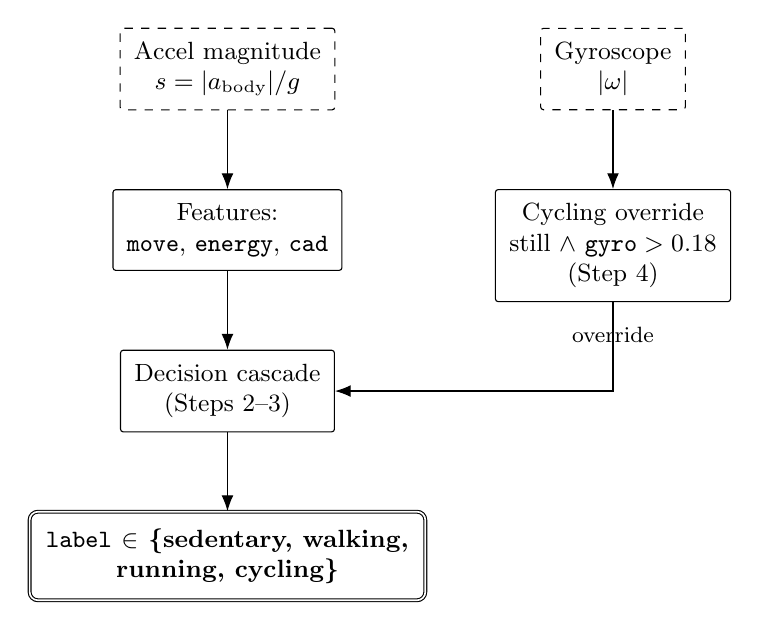
\begin{tikzpicture}[
  node distance=10mm and 26mm,
  box/.style={draw, dashed, rounded corners=1pt, align=center, inner sep=5pt, font=\small},
  op/.style={draw, rounded corners=1pt, align=center, inner sep=5pt, font=\small},
  resultbox/.style={draw, double, rounded corners=3pt, align=center, inner sep=6pt, font=\small\bfseries},
  ar/.style={-{Latex[length=2mm]}}]

  \node[box] (a) {Accel magnitude\\ $s=|a_\text{body}|/g$};
  \node[op, below=of a] (feat) {Features:\\ \texttt{move}, \texttt{energy}, \texttt{cad}};
  \node[op, below=of feat] (casc) {Decision cascade\\ (Steps 2--3)};
  \node[resultbox, below=of casc] (out) {\texttt{label} $\in$ \{sedentary, walking,\\ running, cycling\}};

  \node[box, right=of a] (g) {Gyroscope\\ $|\omega|$};
  \node[op, below=of g] (cyc) {Cycling override\\ still $\wedge\ \texttt{gyro}>0.18$\\ (Step 4)};

  \draw[ar] (a) -- (feat);
  \draw[ar] (feat) -- (casc);
  \draw[ar] (casc) -- (out);
  \draw[ar] (g) -- (cyc);
  \draw[ar] (cyc) |- (casc) node[pos=0.28,above,font=\footnotesize] {override};
\end{tikzpicture}
\caption*{\small Formula flow --- Activity State: a priority decision cascade over
orientation-invariant accelerometer features, with a gyroscope override for cycling.}
\end{figure}

\chapter{Movement Regularity}

\noindent\textbf{Movement Regularity} estimates \textit{how rhythmic and self-repeating
the body's motion is over a short window} --- a smoothness score, not an intensity or a
posture. It is theoretically distinct from \textbf{Activity State} (which measures
\textit{how much} motion and of \textit{what type}) and from \textbf{Postural State}
(which measures orientation relative to gravity). A person can be highly active yet
irregular (stumbling, fidgeting) or barely active yet perfectly regular (a slow steady
walk); regularity is the axis that separates these, so it is a genuinely non-redundant
construct rather than a re-scaling of activity intensity.

\begin{callout}
\textbf{Scope.} This score reports \textit{whether} motion repeats cleanly, not \textit{why}
it does or does not. A low score cannot by itself distinguish a mechanical cause (rough
terrain, an obstacle) from a physiological one (tremor, agitation, fatigue). The score is
only defined while the body is actually moving rhythmically; when the person is still, or
when too few motion cycles fall inside the window, the axis returns \textbf{null} rather
than a misleadingly ``perfect'' value. Resolving the cause of irregularity requires the
Activity State context and the downstream heart-rate / affective layer.
\end{callout}

\section{Theoretical Basis}

The score is the normalized \emph{unbiased autocorrelation} of the acceleration-magnitude
signal at its dominant period. This is the trunk-accelerometry gait-regularity index of
\textbf{Moe-Nilssen \& Helbostad (2004)}: for a walking signal, the value of the normalized
autocorrelation at the stride lag measures how closely one stride reproduces the next, and
the authors note it is cheap enough for portable devices. The parts of the formula
\emph{directly evidenced} by that work are the unbiased-autocorrelation estimator and the
use of its dominant-period peak height as the regularity index. The remaining choices are
\emph{engineering adaptations}, flagged as such below: the clamp to $[0,1]$, the movement
and cycle-count gates, the pocket-placement lag band, and the two-factor confidence.

\begin{itemize}[leftmargin=1.4em]
  \item \textbf{Acceleration magnitude $|a_\text{body}|$} --- gravity-removed body
  acceleration reduced to its Euclidean norm, making the feature orientation-invariant
  (the same rhythm reads identically regardless of how the phone is rotated in the pocket).
  \item \textbf{Unbiased autocorrelation} --- the $1/(N-k)$ normalization corrects the
  end-of-window sample deficit so that longer lags are not artificially damped
  (Moe-Nilssen \& Helbostad, 2004).
  \item \textbf{Smoothness alternatives (not used, cited for completeness)} --- spectral
  arc length SPARC (Balasubramanian et al., 2012) and log dimensionless jerk (LDLJ) are
  established smoothness measures; autocorrelation is chosen here because it is
  period-aware and matches the gait literature.
  \item \textbf{Affective relevance} --- reduced or irregular ambulatory movement is
  associated with agitation and anxiety in actigraphy studies, which motivates exposing
  regularity to the downstream affective read.
\end{itemize}

\section{Input Signals}

\begin{center}
\begin{tabular}{@{}l l >{\raggedright\arraybackslash}p{7.4cm}@{}}
\toprule
\textbf{Signal} & \textbf{Symbol} & \textbf{Description} \\
\midrule
Body acceleration      & $a_\text{body}$ & Gravity-removed 3-axis acceleration (m/s$^2$);
                                            linear-accel sensor, or raw accel low-passed at 0.3\,Hz \\
Acceleration magnitude & $s$             & $|a_\text{body}|/g$, orientation-invariant motion size (g) \\
Dominant lag           & $k^\star$       & Period (samples) of the strongest self-repeat in the window \\
Activity state         & \texttt{ACT}    & Context gate: regularity is only meaningful while walking/running \\
\bottomrule
\end{tabular}
\end{center}

\noindent Window $N = 250$ samples ($5$\,s at $F_s = 50$\,Hz), 50\% overlap. No personal
baseline is required: the score is self-referential within the window.

\section{Rule Formula}

\begin{rulebox}{RULE-MR}{Movement Regularity Score}
\textbf{Step 1 --- Magnitude and detrend:}
\[ s(t) = \frac{|a_\text{body}(t)|}{g}, \qquad x(t) = s(t) - \overline{s}, \qquad
   \text{movement} = \std(s). \]

\textbf{Step 2 --- Unbiased, normalized autocorrelation} (lags $k = 0\dots K$, $K=100$):
\[ r(k) = \frac{1}{N-k}\sum_{t=0}^{N-1-k} x(t)\,x(t+k), \qquad
   \rho(k) = \frac{r(k)}{r(0)}. \]

\textbf{Step 3 --- Dominant period} (argmax over the stride band, not the first peak):
\[ k^\star = \operatorname*{arg\,max}_{k\in[10,100]} \rho(k), \qquad
   n_\text{cyc} = \frac{N}{k^\star}. \]

\textbf{Step 4 --- Score:}
\[ R = \clamp\big(\rho(k^\star),\,0,\,1\big). \]

\textbf{Step 5 --- Validity gate} (return \textbf{null} instead of a score if):
\[ \text{movement} < 0.051\text{ g}\ \ (\text{low\_movement}) \quad\text{or}\quad
   n_\text{cyc} < 3.5\ \ (\text{insufficient\_cycles}). \]

\boxform{ R \in [0,1] \ \text{ if valid, else null} }

\smallskip
\textit{Example:} steady pocket walk, $\std(s)=0.37$\,g, $k^\star=55$ ($\approx0.9$\,Hz
stride), $\rho(k^\star)=0.71$, $n_\text{cyc}=250/55=4.5$. Both gates pass
$\Rightarrow R = 0.71$ (``rhythmic'').
\end{rulebox}

\section{Parameter Notes}

\noindent\textbf{Regularity estimator} {\footnotesize\textsc{[theory]}}\textbf{.}
The score itself --- the normalized unbiased autocorrelation at the dominant period --- is
taken directly from the Moe-Nilssen \& Helbostad (2004) trunk-gait index. It is the one number
here that comes straight from published theory; everything else is a gate or a confidence
around it.

\noindent\textbf{Lag band $[10,100]$ samples} {\footnotesize\textsc{[conv]}}\textbf{.}
At $50$\,Hz this covers stride periods $0.2$--$2.0$\,s ($0.5$--$5$\,Hz), the plausible human
cadence range. Taking the \emph{argmax} over the whole band (rather than the first
prominence peak) is deliberate: on pocket data the autocorrelation has strong sub-stride
harmonics, and the first peak grabs a half-stride and inverts the rank ordering. This is the
FIX~2 correction re-derived during the chest$\rightarrow$pocket convergence test.

\noindent\textbf{Movement floor $0.051$\,g} {\footnotesize\textsc{[design]}}\textbf{.}
Below this, magnitude variation is sensor noise, not motion, and the autocorrelation of
noise produces a spurious high peak. The value is the chest-derived $0.5$\,m/s$^2$ floor
re-expressed in g ($0.5/9.81$); expressing it in stream units was FIX~1 of the convergence
test.

\noindent\textbf{Minimum cycles $3.5$ strides} {\footnotesize\textsc{[conv]}}\textbf{.}
Fewer than $\sim$3--4 repeats in the window makes a ``regularity'' estimate statistically
meaningless. $3.5$ stride-periods is the gait-literature adequacy minimum, re-expressed for
the argmax-selects-stride convention on pocket placement.

\noindent\textbf{Prominence saturation $P_\text{full}=1.5$} {\footnotesize\textsc{[design]}}\textbf{.}
The peak prominence at which the confidence prominence term reaches $1$; a chosen saturation
point, not a measured quantity.

\noindent\textbf{Fusion method.}
There is \emph{no} multi-signal fusion in the score itself --- it is a single autocorrelation
read. Fusion appears only in the \emph{confidence} (\S\,Confidence), which combines two
\emph{independent} adequacy factors (enough cycles, and a prominent peak) as a geometric
mean, so that either factor being weak pulls confidence down. The score's \emph{separation}
(not an absolute accuracy) was validated on PAMAP2/MotionSense; the gates and confidence are
\textsc{design} choices tuned to keep noise from scoring as rhythm. Tag meanings are defined
in the Key Terms front-matter.

\section{Confidence}

\noindent\textbf{Step C1 --- Cycle adequacy} (how far past the minimum the window sits):
\[ c_\text{cyc} = \clamp\!\left(\frac{n_\text{cyc}-3.5}{5.0-3.5},\,0,\,1\right). \]

\noindent\textbf{Step C2 --- Peak prominence} ($p$ = prominence of the peak at $k^\star$;
$1.5$ = saturation):
\[ c_\text{prom} = \clamp\!\left(\frac{p}{1.5},\,0,\,1\right). \]

\noindent\textbf{Step C3 --- Final confidence} (geometric mean of the two):
\boxform{ \text{conf} = \sqrt{\,c_\text{cyc}\cdot c_\text{prom}\,} }

\noindent\emph{Confidence ceiling / caveat.} This axis reports no labelled accuracy by
design --- it is validated by \emph{separation} (rank-ordering rhythmic above irregular
above still), not against a ground-truth ``regularity'' label, which does not exist in the
datasets. Confidence therefore expresses \emph{internal signal quality} (enough clean
cycles), not calibrated correctness, and should not be read as a probability.

\section{Interpretation Scale}

\begin{center}
\begin{tabular}{@{}lll@{}}
\toprule
\textbf{Score} & \textbf{Level} & \textbf{Meaning} \\
\midrule
0.0--0.2 & Erratic          & Motion present but not self-repeating (stumbling, fidgeting) \\
0.2--0.4 & Low regularity   & Weak, inconsistent rhythm \\
0.4--0.6 & Moderate         & Discernible but imperfect rhythm \\
0.6--0.8 & Rhythmic         & Clear, steady periodic motion (typical walking) \\
0.8--1.0 & Highly regular   & Metronomic, strongly self-repeating (steady running/pace) \\
\midrule
\textit{null} & Not applicable & Still, or too few cycles --- no rhythm to score \\
\bottomrule
\end{tabular}
\end{center}

\section{Context Applicability}

\begin{callout}
\textbf{Target context:} on-body (pocket / trunk) accelerometry during \emph{sustained
locomotion}. The score is most reliable when the Activity State is walking or running.
\end{callout}

\begin{center}
\begin{tabular}{@{}>{\raggedright\arraybackslash}p{5.6cm} c c >{\raggedright\arraybackslash}p{3.6cm}@{}}
\toprule
\textbf{Context} & \textbf{$|a_\text{body}|$} & \textbf{cycles $\geq 3.5$} & \textbf{Reliable?} \\
\midrule
Walking / running (pocket or trunk) & Yes & Yes & Yes --- full \\
Cycling / non-gait rhythmic motion  & Yes & Partial & Partial (period may fall outside band) \\
Standing / sitting / lying          & No  & No  & No --- returns null \\
\bottomrule
\end{tabular}
\end{center}

\noindent\textbf{Scientific boundary.} Even with ideal data, the score cannot attribute
\emph{cause}: it measures the presence of rhythm, not its origin, so it approximates
``movement smoothness'' rather than directly measuring any affective or neuromotor state.
On PAMAP2 (chest) the score separates rhythmic from irregular-but-moving activity, so it is
not merely a movement detector; on the pocket, only the still-versus-rhythmic contrast is
confirmed so far, and rhythmic-versus-irregular-moving on the pocket is owed to own-phone data.

\section{Worked Example: Steady Commute Walk}

\noindent\textit{Scenario.} A user walks to a bus stop at a relaxed, even pace, phone in the
front trouser pocket. Over one $5$\,s window the pipeline extracts:

\begin{center}
\begin{tabular}{@{}ll@{}}
\toprule
\textbf{Signal} & \textbf{Value} \\
\midrule
$\std(s)$ (movement)        & $0.37$\,g \\
Dominant lag $k^\star$      & $55$ samples ($\approx 0.9$\,Hz stride) \\
$\rho(k^\star)$             & $0.71$ \\
Peak prominence $p$         & $0.60$ \\
\bottomrule
\end{tabular}
\end{center}

\noindent\textbf{Step-by-step:}
\begin{align*}
n_\text{cyc} &= 250/55 = 4.5 \;(\geq 3.5,\ \text{movement } 0.37>0.051 \Rightarrow \text{valid})\\
R            &= \clamp(0.71,0,1) = \mathbf{0.71}\\
c_\text{cyc} &= \clamp\big((4.5-3.5)/1.5,0,1\big) = 0.67\\
c_\text{prom}&= \clamp(0.60/1.5,0,1) = 0.40\\
\text{conf}  &= \sqrt{0.67\cdot 0.40} = \mathbf{0.52}
\end{align*}

\begin{callout}
\textbf{Interpretation:} $R = 0.71$ falls in the \emph{Rhythmic} band --- a clean, steady
walking cadence. The dominant driver is the high autocorrelation peak ($\rho=0.71$);
confidence is moderate ($0.52$), held down by the modest peak prominence rather than by
too few cycles.
\end{callout}

\section{Implementation Notes}

\begin{itemize}[leftmargin=1.4em]
  \item \textbf{Window.} $250$ samples ($5$\,s) at $50$\,Hz, 50\% overlap; magnitude is
  read from the same rolling buffer the other 5\,s axes use.
  \item \textbf{Fallback behavior.} No accel/linear stream $\rightarrow$ null. A window that
  is $>50\%$ bad samples ($\mathrm{NaN}$ or $>16$\,g), or whose first sample is bad,
  $\rightarrow$ null (\texttt{window\_unreliable}); shorter gaps are forward-filled. If
  \texttt{scipy} is unavailable the score still computes; only the prominence confidence
  factor degrades.
  \item \textbf{Relationship to other chapters.} Gated by \textbf{Activity State} --- a
  regularity number is only surfaced while \texttt{ACT} indicates locomotion; on its own,
  regularity cannot tell moving-irregular from still, which is why the two axes are read
  together.
  \item \textbf{Validation status.} No labelled accuracy by design (there is no ground-truth
  regularity label), so validation is by \emph{separation}. On PAMAP2 chest, rhythmic vs
  irregular ROC-AUC $0.99$ (per-subject median $0.99$, all 8 evaluable subjects $\geq 0.97$).
  It transfers \emph{frozen} to two further datasets and sensor types (table below).
  \textbf{And it is regularity, not movement:} restricted to \emph{moving} windows --- so
  ``moving vs still'' cannot explain the split --- rhythmic vs irregular-but-moving
  (vacuuming, ironing) still separates at ROC-AUC $0.99$: vacuuming moves yet scores
  ${\sim}0.25$ while walking scores ${\sim}0.94$ (regularity correlates with movement only
  ${\sim}{+}0.5$). This movement-control exists only on PAMAP2; the pocket version is owed to
  own-phone data.
\end{itemize}

\begin{center}
\begin{tabular}{@{}>{\raggedright\arraybackslash}p{2.4cm} >{\raggedright\arraybackslash}p{3.6cm} >{\raggedright\arraybackslash}p{3.4cm} l@{}}
\toprule
\textbf{Dataset} & \textbf{Placement / sensor} & \textbf{Contrast} & \textbf{ROC-AUC} \\
\midrule
PAMAP2      & chest, research IMU        & rhythmic vs irregular & $0.99$ \\
MotionSense & pocket, phone              & rhythmic vs still     & $0.96$ \\
HHAR        & waist/hand, phone + watch  & walking vs still      & $0.98$ \\
\bottomrule
\end{tabular}
\end{center}

\noindent{\footnotesize MotionSense/HHAR have no irregular-but-moving activity, so
cross-dataset confirms rhythmic $>$ still only. HHAR must be resampled \emph{within gap-free
spans}: its heterogeneous sampling, interpolated across gaps, otherwise fakes periodicity.}

% ---- Formula flow diagram ----
\begin{figure}[h]
\centering
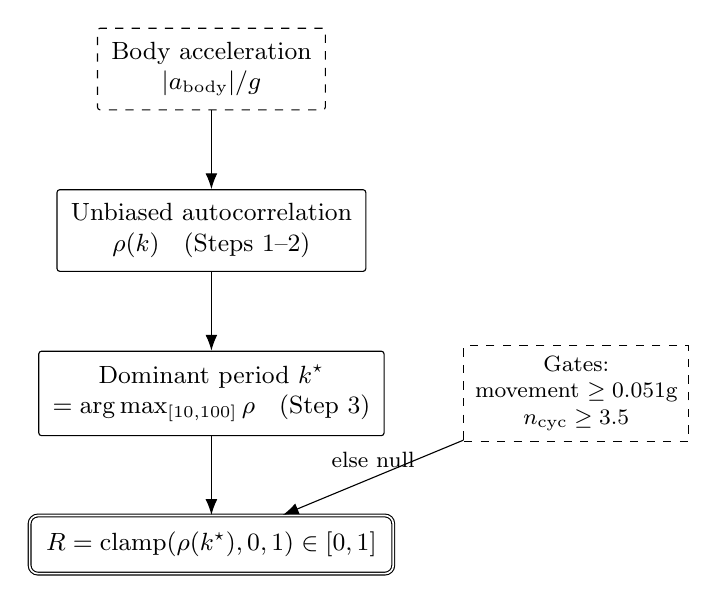
\begin{tikzpicture}[
  node distance=10mm and 14mm,
  box/.style={draw, dashed, rounded corners=1pt, align=center, inner sep=5pt, font=\small},
  op/.style={draw, rounded corners=1pt, align=center, inner sep=5pt, font=\small},
  resultbox/.style={draw, double, rounded corners=3pt, align=center, inner sep=6pt, font=\small\bfseries},
  gate/.style={draw, dashed, align=center, inner sep=4pt, font=\footnotesize},
  ar/.style={-{Latex[length=2mm]}}]

  \node[box] (in) {Body acceleration\\ $|a_\text{body}|/g$};
  \node[op, below=of in] (ac) {Unbiased autocorrelation\\ $\rho(k)$ \; (Steps 1--2)};
  \node[op, below=of ac] (peak) {Dominant period $k^\star$\\ $=\arg\max_{[10,100]}\rho$ \; (Step 3)};
  \node[gate, right=10mm of peak] (g) {Gates:\\ movement $\geq 0.051$g\\ $n_\text{cyc}\geq 3.5$};
  \node[resultbox, below=of peak] (score) {$R=\clamp(\rho(k^\star),0,1) \in [0,1]$};

  \draw[ar] (in) -- (ac);
  \draw[ar] (ac) -- (peak);
  \draw[ar] (peak) -- (score);
  \draw[ar] (g) -- (score) node[midway,above,font=\footnotesize] {else null};
\end{tikzpicture}
\caption*{\small Formula flow --- Movement Regularity: one orientation-invariant input,
period-aware autocorrelation, a validity gate, and a $[0,1]$ score.}
\end{figure}

% \include{chapters/postural_state}
% \include{chapters/locomotion_state}
% \include{chapters/overall_state}

\end{document}
